\chapter{Conclusions}
\label{chapter:conclusions}

\section{Summary of Findings}
\label{section:summary_of_findings}

\subsection{Overview of the study objectives and what was undertaken}

This study investigated the extent to which machine-learned interatomic potentials (MLPs), specifically the MACE
framework, can replicate interface favourability rankings computed via density functional theory (DFT) across various
group-IV semiconductor systems, including carbon (C), silicon (Si), germanium (Ge), and tin (Sn). The project involved
automated structure generation with ARTEMIS, interface relaxation via both DFT and MLP, and evaluation of rank
preservation using statistical metrics including Spearman and Kendall correlations, as well as Top-N overlap.

\subsection{Recap of major results:}

\subsubsection{MLP vs DFT rank alignment}

The agreement between MLP and DFT was found to be system-dependent. MLPs performed well for Ge and Sn systems,
achieving high rank correlation and overlap with DFT rankings. For Si, alignment was significantly poorer, with
frequent rank reversals and diminished correlation metrics.

\begin{figure}[h]
    \centering
    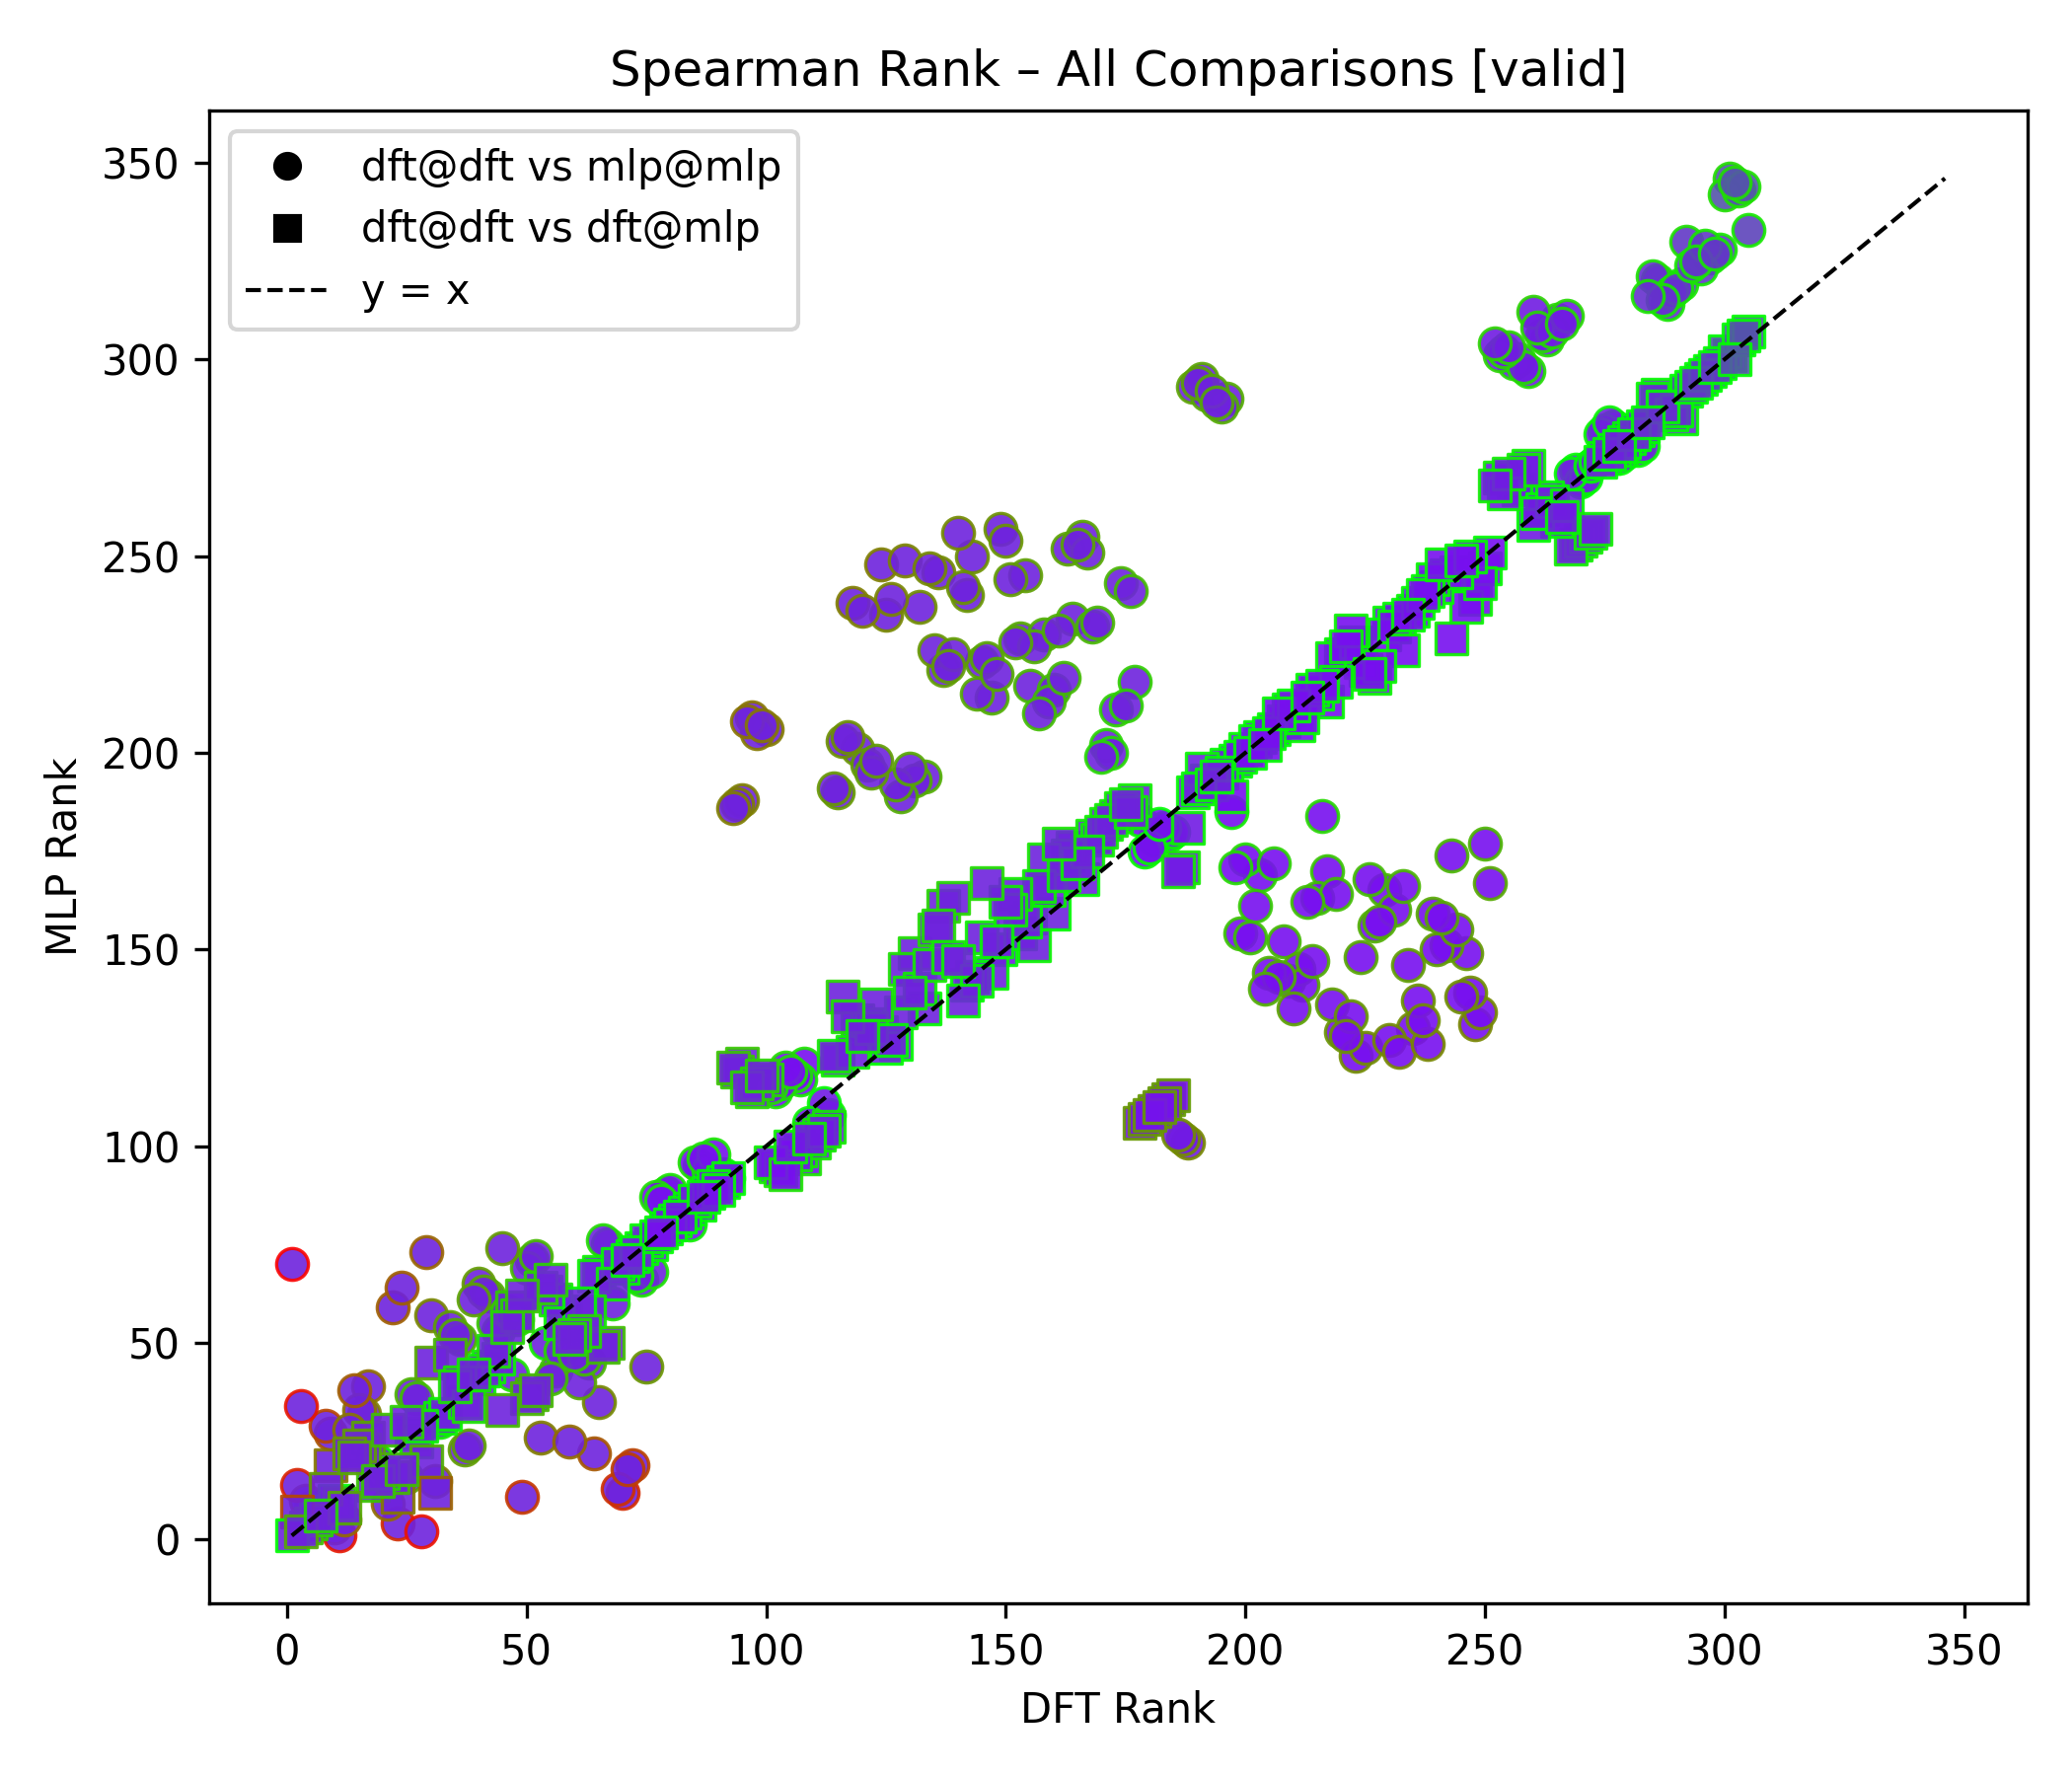
\includegraphics[width=0.7\textwidth]{analysis/plots/results_lower_Si_spearman_all_comparisons_valid.png}
    \caption{Spearman rank correlation for Si interfaces.}
\end{figure}

\subsubsection{System-specific performance (C, Si, Ge, Sn)}

Carbon results remain incomplete and thus inconclusive. Silicon systems exhibited persistent discrepancies between MLP
and DFT rankings. Germanium and tin interfaces, by contrast, showed favourable agreement, with strong rank preservation
and good Top-N screening utility.

\begin{table}[h]
    \centering
    \caption{Performance metrics for Si interfaces from \texttt{analysis/stats_upper_Si.csv}.}
    \begin{tabular}{lcccccc}
        Comparison & Spearman & Kendall & RMSE & MAE & Top-10 Overlap \\
        \hline
        DFT@DFT vs MLP@MLP & 0.46 & 0.31 & 7.48 & 3.36 & 3 \\
    \end{tabular}
\end{table}

\subsubsection{Value of cross-evaluation (e.g. DFT@MLP)}

Although direct MLP-on-DFT-relaxed structure evaluations (MLP@DFT) were not included due to computational cost, the
study revealed that relaxation--evaluation consistency (e.g. MLP@MLP vs DFT@DFT) influences error, and future
cross-evaluation may further clarify error sources.

% Placeholder for future figure showing relaxation-evaluation matrix comparisons.

\section{Interface Rank Preservation}
\label{section:interface_rank_preservation}

\subsection{Effectiveness of MLPs in reproducing DFT interface energetics}

Absolute energy discrepancies were evident but secondary to the study goal. More relevant was the preservation of
ranking. For Ge and Sn, MLPs captured the energetic hierarchy of interfaces with reasonable fidelity, while for Si, the
energetic ordering was often disrupted.

\begin{figure}[h]
    \centering
    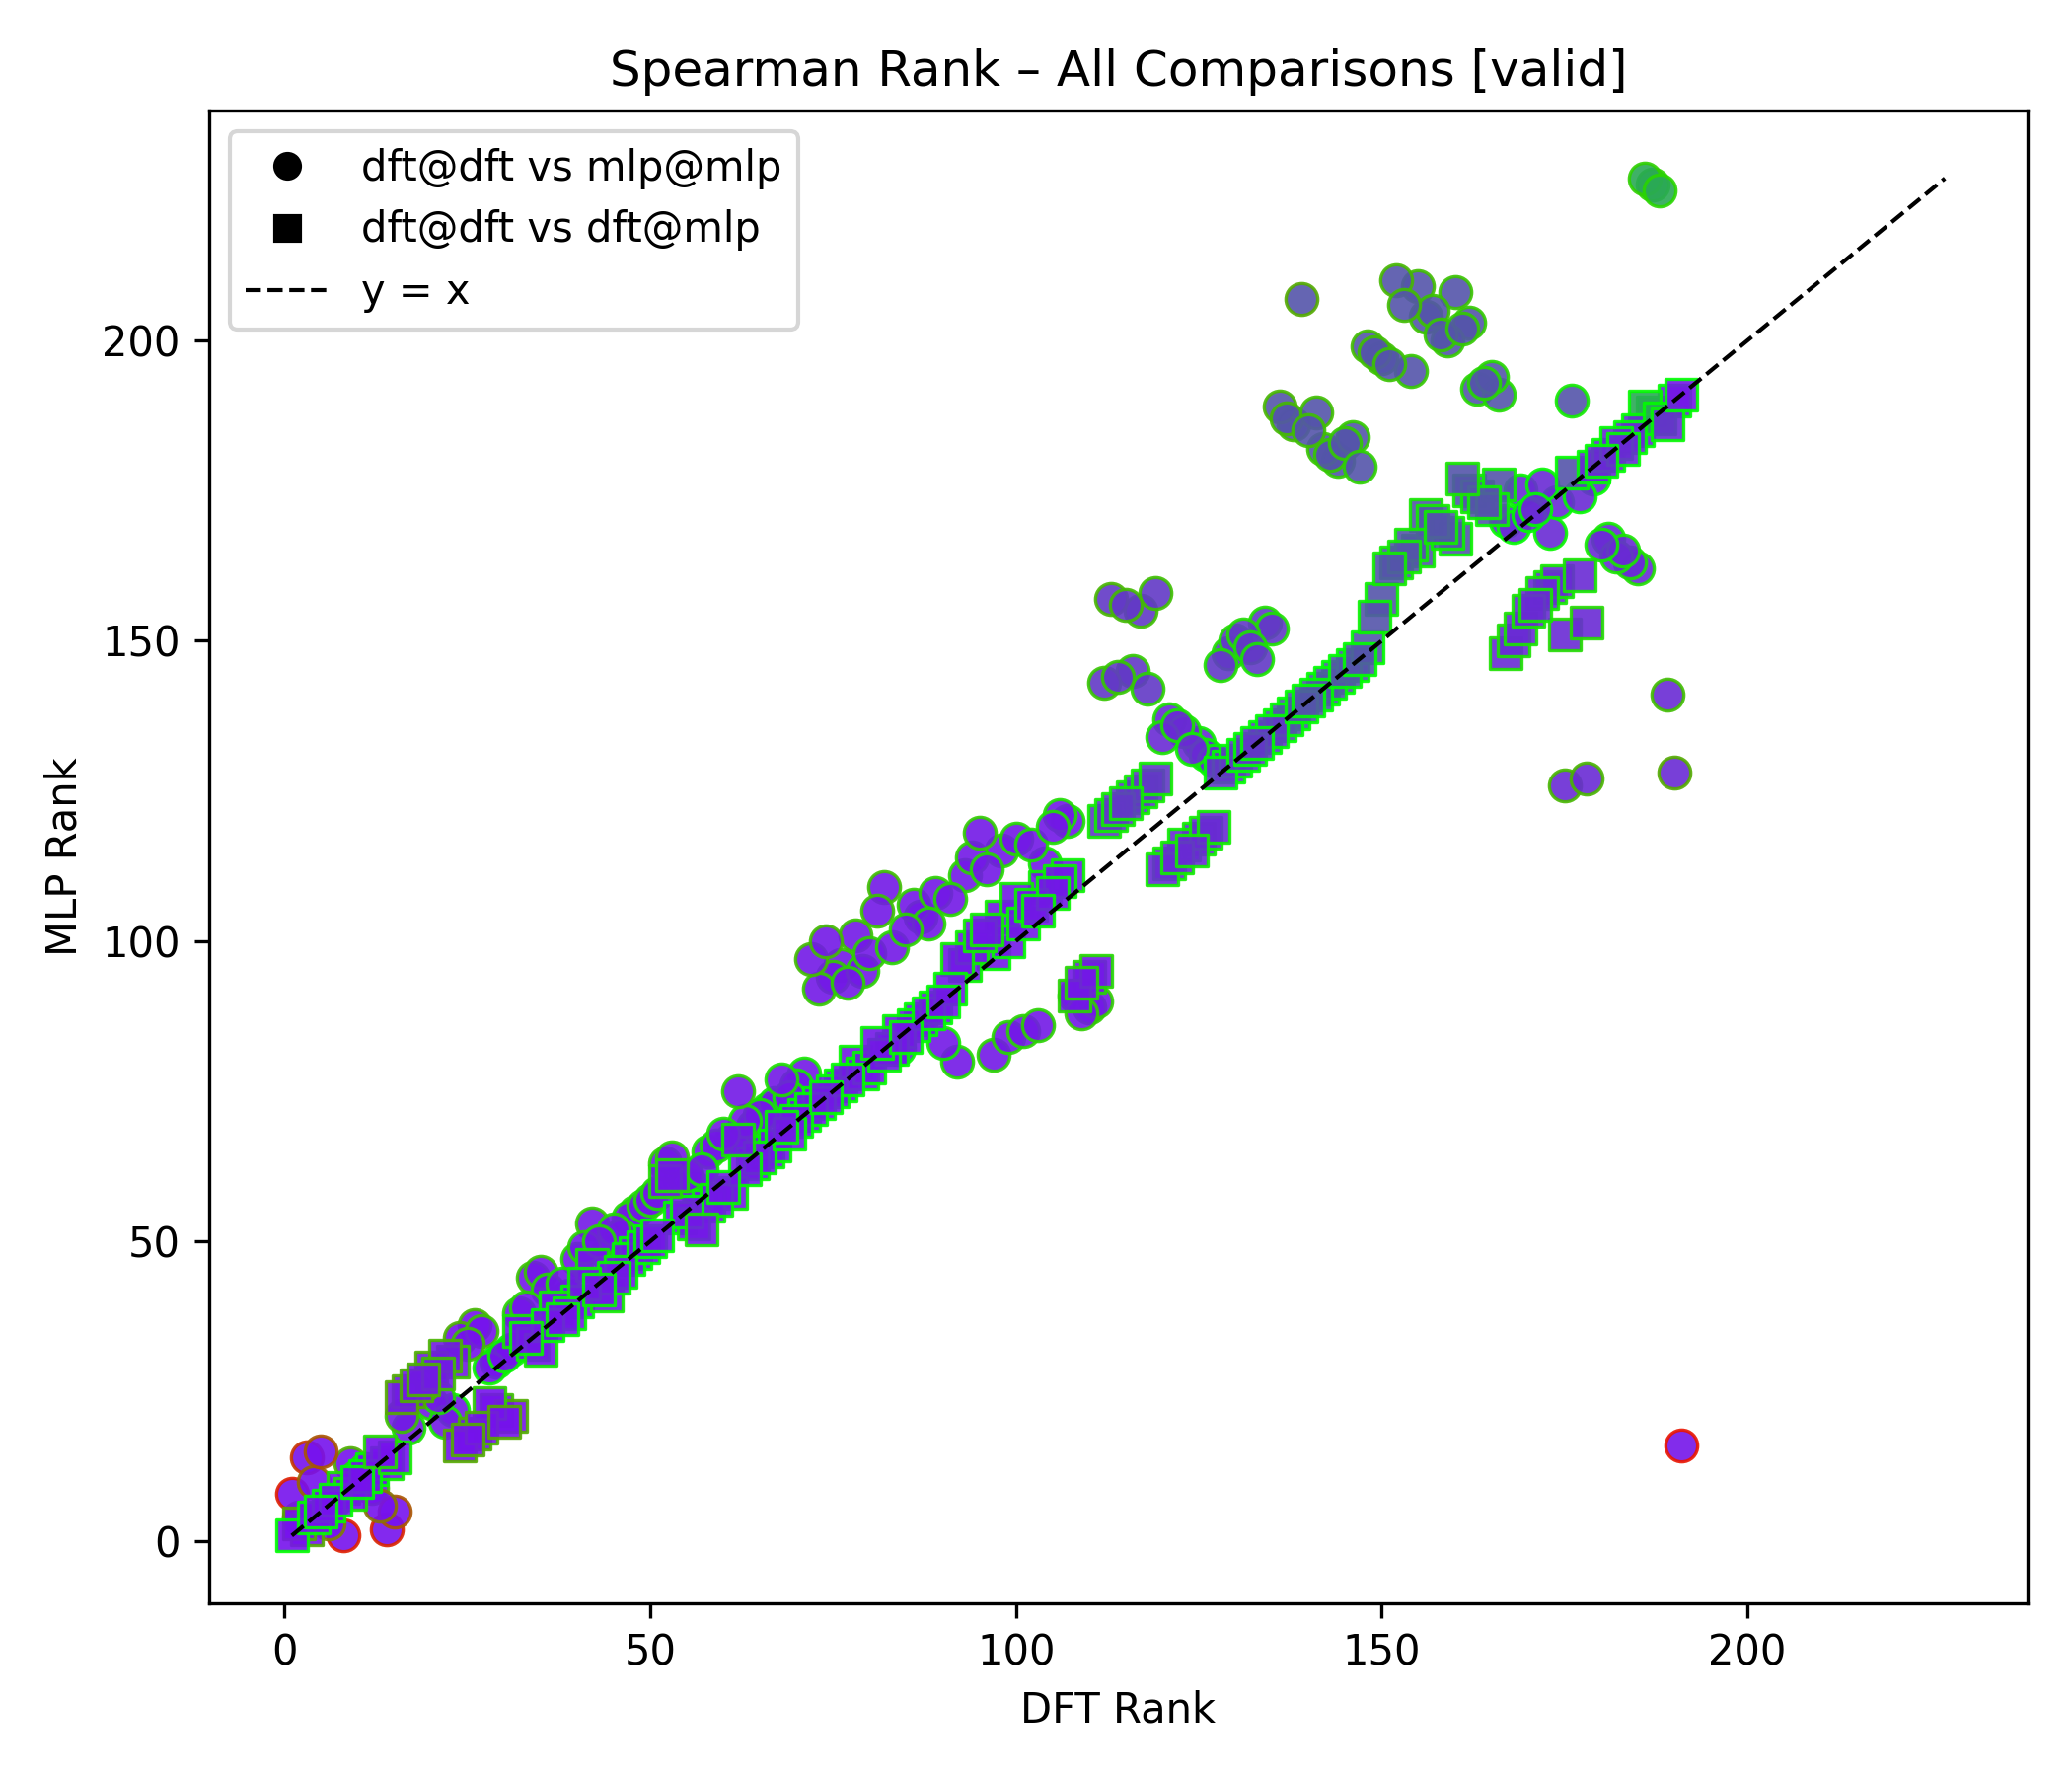
\includegraphics[width=0.7\textwidth]{analysis/plots/results_lower_Ge_spearman_all_comparisons_valid.png}
    \caption{Spearman correlation for Ge interfaces.}
\end{figure}

\subsection{Top-N performance and rank correlations}

Top-N overlap and Spearman/Kendall rank statistics highlighted the utility of MLPs in screening contexts. Even where
absolute energies were misaligned, the preservation of top candidate rankings proved robust in Ge and Sn systems.

\begin{figure}[h]
    \centering
    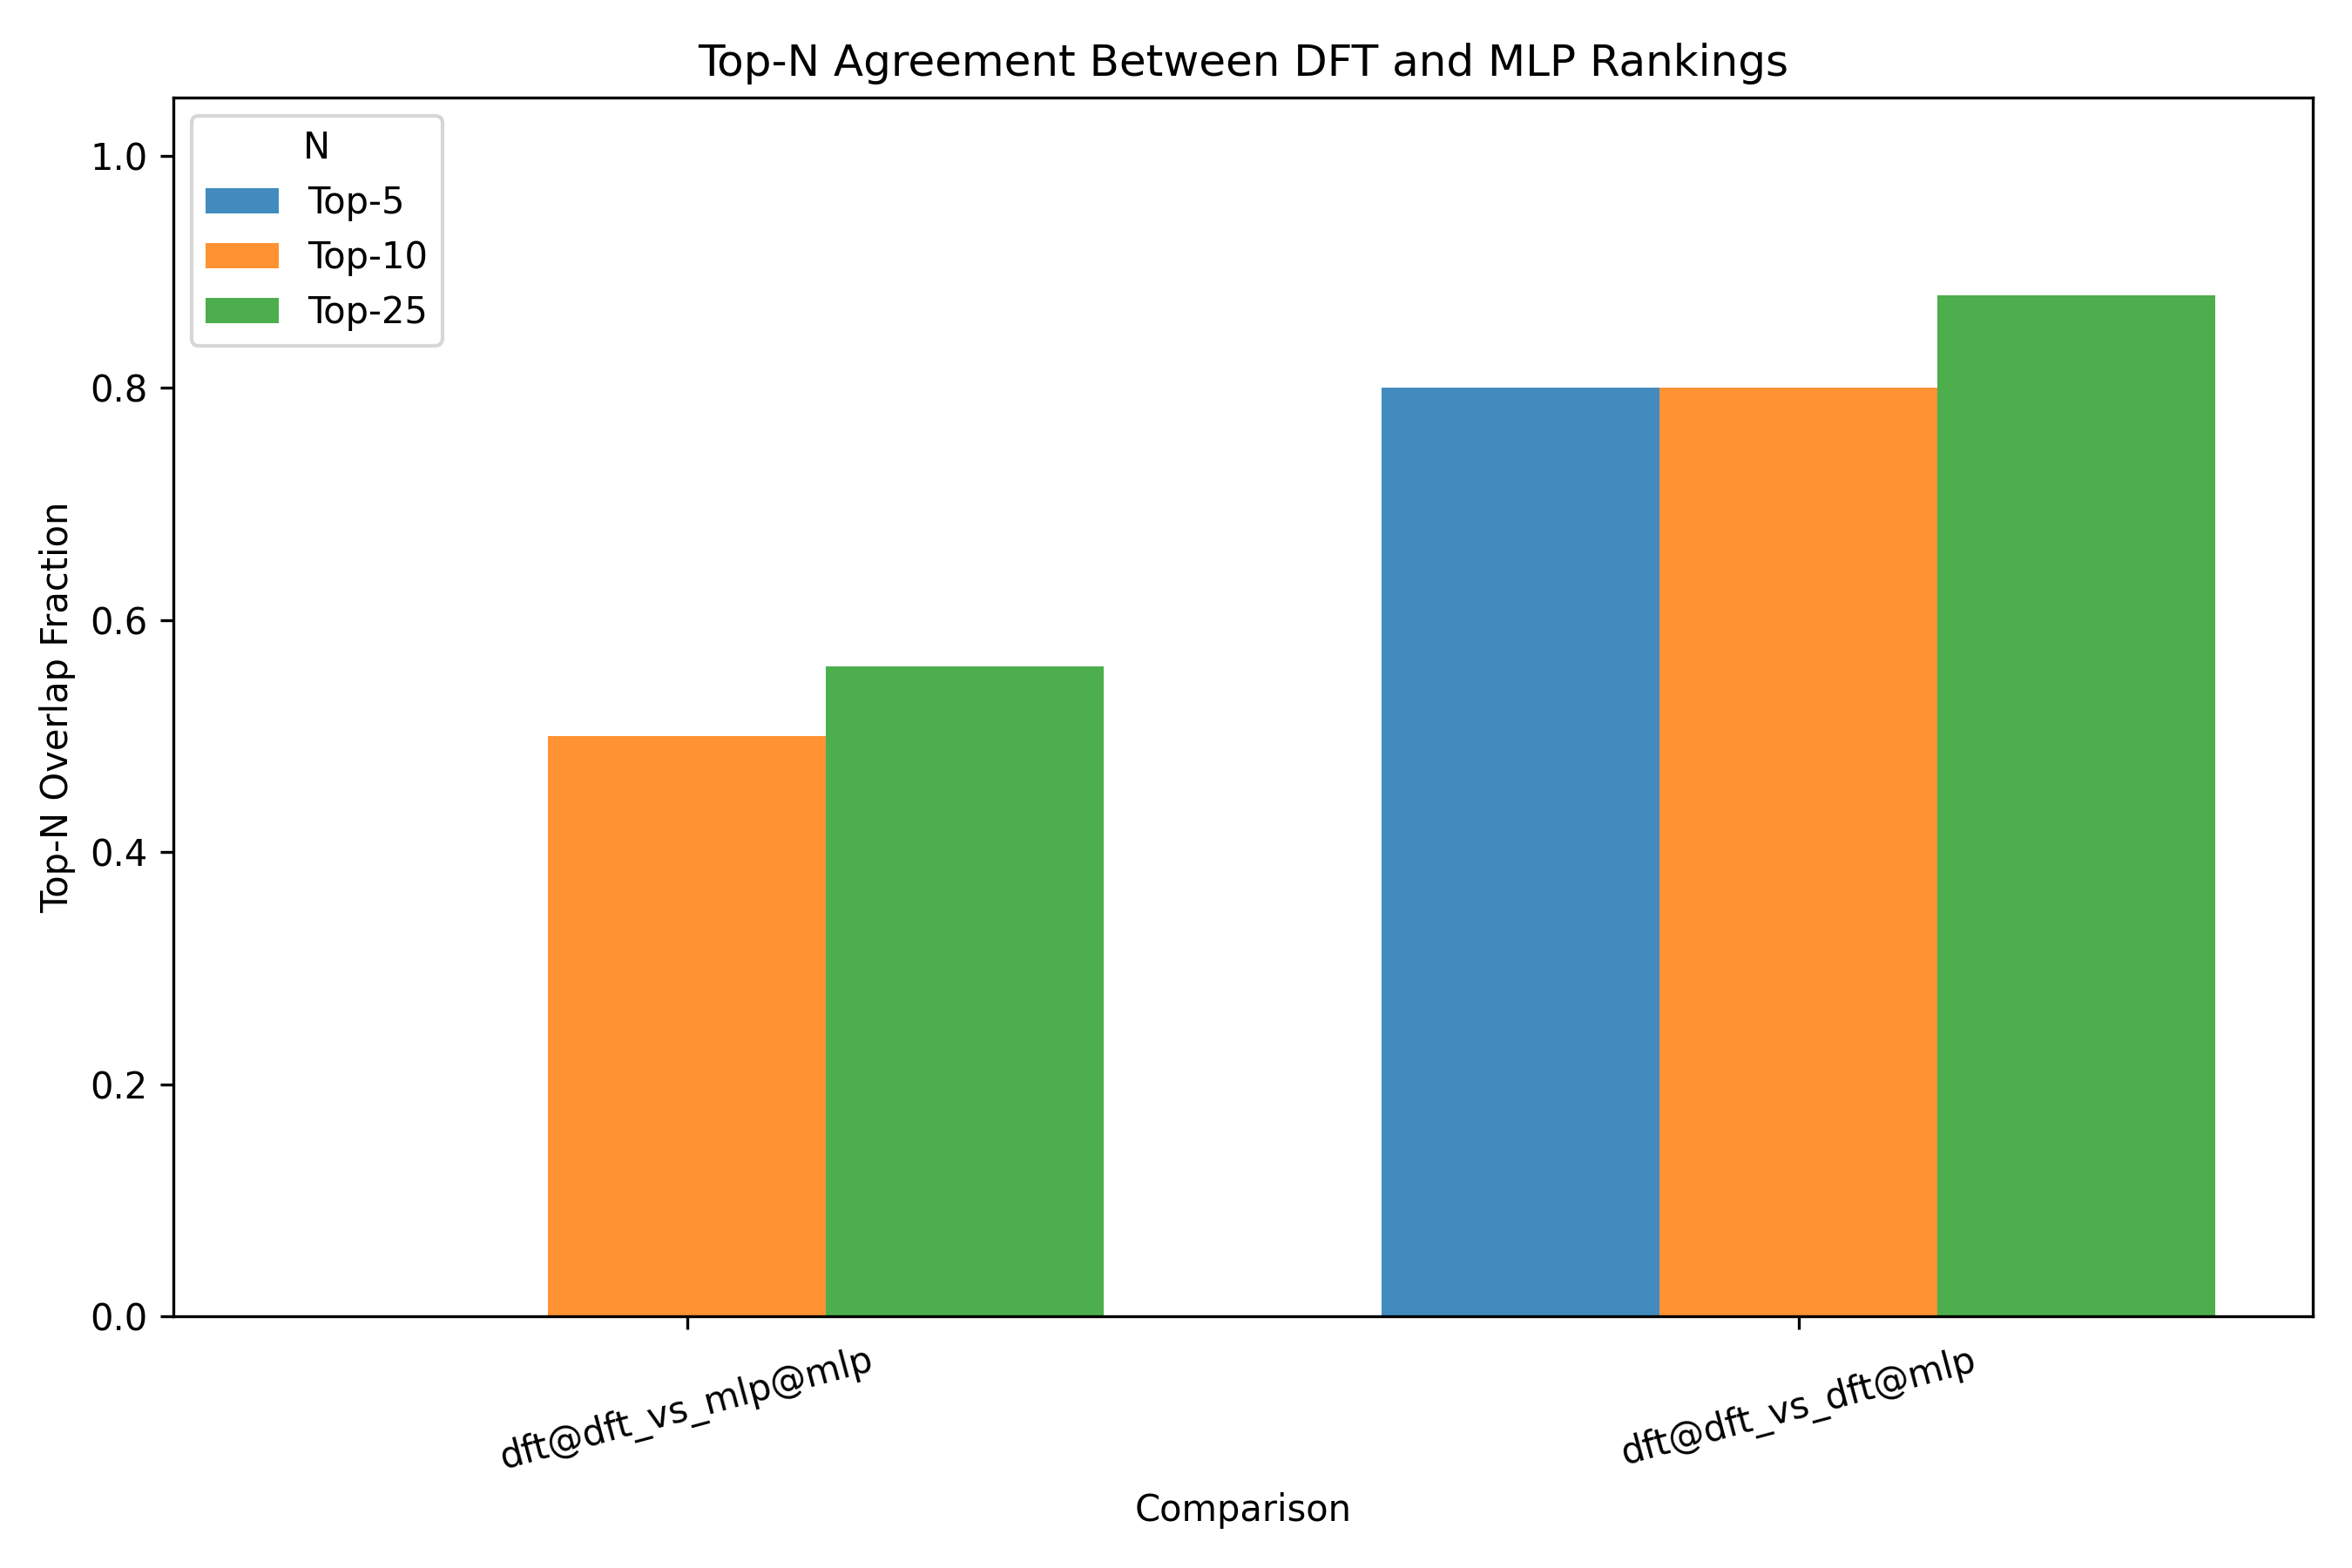
\includegraphics[width=0.7\textwidth]{analysis/plots/results_lower_Si_topn_overlap.png}
    \caption{Top-\textit{N} overlap for Si interfaces.}
\end{figure}

\subsection{Strengths vs weaknesses}

MLPs offer clear advantages in computational speed and can safely be used for preliminary screening in certain systems.
However, their generalisation is inconsistent, especially in covalently bonded systems like Si. Without targeted
retraining, MLPs may mislead in these cases.

% Equation suggestion: O(n) comparison of DFT vs MLP computational cost per electron.

\section{Insights from Work Undertaken}
\label{section:insights_from_work}

\subsection{What was learned from each system}

\subsubsection{Carbon (C) – data incompleteness and implications}

The carbon dataset remains incomplete and cannot yet support definitive conclusions. Preliminary indications suggest
that strong bonding and limited configurational diversity may pose challenges analogous to those observed in Si.

\subsubsection{Silicon (Si) – persistent poor rank correlation}

Across all iterations, Si consistently exhibited poor MLP--DFT agreement. This suggests intrinsic modelling
difficulties rather than statistical noise. The failures appear systematic, reinforcing the need for targeted
improvements.

\subsubsection{Germanium (Ge) and Tin (Sn) – favourable MLP--DFT agreement}

For both Ge and Sn, MLPs reliably preserved DFT-derived rankings. These systems are likely well-represented in the MACE
training dataset, and their more metallic bonding character may aid accurate regression of energies.

\subsection{Contrast perfect alloys vs heterostructures}

Perfect alloy systems showed tighter rank correlation and lower error dispersion than heterostructures.

\begin{table}[h]
    \centering
    \caption{Comparison of MLP performance on perfect alloys and heterostructures.}
    \begin{tabular}{lccc}
        System & Spearman & Kendall & Top-10 Overlap \\
        \hline
        Perfect Alloys & 1.00 & 1.00 & 6 \\
        Ge|Si Heterostructure & 0.73 & 0.55 & 6 \\
    \end{tabular}
\end{table}

\section{Challenges in Modelling Silicon Interfaces}
\label{section:challenges_in_modelling_silicon_interfaces}

\subsection{Discussion of why MLPs fail for Si:}

\subsubsection{Local bonding features?}

MLPs may struggle with the directional covalent bonding and short bond lengths characteristic of Si. These features
introduce sensitivity to structural distortions that are difficult to learn from sparse data.

\subsubsection{Underrepresented environments in training?}

It is likely that the MACE training set lacks sufficient coverage of interfacial Si environments, especially those with
reconstructed surfaces and strained bonds.

\subsection{Open questions}

\subsubsection{Is Si anomalous, or are MLP limitations broader?}

The current data cannot confirm whether Si represents a broader warning about MLP application or a special case.
Additional experiments with other covalently bonded systems are required to determine generalisability.

\section{Broader Lessons and Limitations}
\label{section:broader_lessons_and_limitations}

\subsection{When can MLPs be trusted for interface screening?}

MLPs appear trustworthy when used to rank candidates in systems whose bonding and local structures are well-represented
in the training data. Screening workflows benefit most from MLPs in Ge and Sn contexts.

\subsection{Necessity of retraining, delta-correction, or hybrid workflows}

The results support the need for delta-correction approaches, particularly for challenging systems like Si. Hybrid
workflows that combine MLP-based pre-screening with DFT confirmation for top candidates offer a balanced path forward.

% Placeholder for conceptual diagram of hybrid MLP–DFT workflow.

\subsubsection{Importance of careful benchmarking}

This study underscores the importance of benchmarking MLPs using rank-based metrics, not just energy errors. Rank
preservation aligns more closely with practical use in structure discovery.

\section{Concluding Remarks}
\label{section:concluding_remarks}

\subsection{What this work contributes to the field of ML-accelerated interface modelling}

This work demonstrates that while current general-purpose MLPs like MACE can preserve interface rankings in selected
systems, their utility is uneven. The study identifies conditions under which MLPs can be safely used and highlights
where caution or additional training is warranted.

\subsection{Final note on significance for device and materials design}

By enabling rapid, large-scale screening of interfacial configurations in certain systems, this work lays the
groundwork for accelerated discovery of novel interfaces. Continued refinement of MLPs and integrated hybrid workflows
will be essential to extend this capability to the full range of materials relevant for device engineering.

% Final figure suggestion: Summary infographic showing findings, limitations, and future directions.
